\documentclass{beamer}
\usetheme{metropolis} % Use metropolis theme

\title{ECON 3818: Introduction to Statistics with Computer Applications}
%\subtitle
\date{\today}
\author{Kyle Butts}

\definecolor{blue}{RGB}{0,114,178}
\definecolor{red}{HTML}{EB0E09}
\definecolor{yellow}{RGB}{240,228,66}
\definecolor{green}{RGB}{0,158,115}
\definecolor{maroon}{HTML}{AF3335}
\definecolor{purple}{HTML}{7E90B8}

\definecolor{mybackground}{HTML}{ECECEC}
\setbeamercolor{background canvas}{bg= mybackground}

\definecolor{buff-gold}{HTML}{CFB87C}
\definecolor{buff-grey}{HTML}{565A5C}
\definecolor{buff-lightgrey}{HTML}{A2A4A3}
\definecolor{buff-black}{HTML}{000000}

\setbeamercolor{alerted text}{fg=buff-gold!80!black}
\setbeamercolor{frametitle}{bg=buff-black}
\setbeamercolor{title}{fg=buff-grey}
\setbeamercolor{button}{bg=buff-gold}

% Allow to remove indent w/ \begin{itemize}[leftmargin= *]
\usepackage{enumitem}
\setlist[itemize]{label= \textbullet}

% \usepackage[libertine]{newtxmath}
\usepackage{longtable}
\usepackage{booktabs}
\usepackage{enumitem}


\begin{document}

% Title Page ---------------------------------------
\maketitle




% Chapter 15 ---------------------------------------
\section{Chapter 15: Parameters and Statistics}

\begin{frame}{Parameters and Statistics}
	We have discussed using sample data to make inference about the population.  In particular, we will use sample \alert{statistics} to make inference about population \alert{parameters}.
	
    \begin{definition}[Parameter]
        \vspace{2.5mm}
		A \alert{parameter} is a number that describes the population. In practice, parameters are unknown because we cannot examine the entire population.
	\end{definition}
	
    \begin{definition}[Statistic]
        \vspace{2.5mm}
		A \alert{statistic} is a number that can be calculated from sample data without using any unknown parameters. In practice, we use statistics to estimate parameters.
	\end{definition}
\end{frame}


\begin{frame}{Greek Letters and Statistics}
	\begin{columns}[onlytextwidth] % align columns

		\begin{column}{.5\textwidth}
			\begin{center}
				\textbf{Greek Letters (Parameters)}
			\end{center}

			\begin{itemize}
				\item Greek letters like $\mu$ and $\sigma^2$ represent the truth about the population.
			\end{itemize}
		\end{column}%
		\hfill%

		\begin{column}{.5\textwidth}
			\begin{center}
				\textbf{Latin Letters (Statistic)}
			\end{center}

			\begin{itemize}
				\item Latin lettes like $\bar{x}$ and $s^2$ are calculations that represent guesses (estimates) at the population values.
			\end{itemize}
		\end{column}%
	\end{columns}
	
	\vspace{10mm}
	The goal for the class is for the latin letters to be good guesses for the greek letters:

	\[ 
		\text{Data} \longrightarrow \text{Calculation} \longrightarrow \text{Estimates} \longrightarrow^{hopefully!} \text{Truth}
	\]
	\[
		X \longrightarrow 1/n \sum_{i=1}^n X_i \longrightarrow \bar{x} \longrightarrow^{hopefullly!} \mu
	\]
\end{frame}

\begin{frame}{Examples of Parameters}
	Some parameters of distributions we've encountered are
	\begin{itemize}
		\item $n$ and $p$ in $X\sim B(n,p)$ where 
		\begin{align*}
			P(X=x)={n \choose x} p^x \left(1-p\right)^{n-x} 
		\end{align*}
		\item $a$ and $b$ in $X\sim U(a,b)$
		\begin{align*}
			f(x)=\frac{1}{b-a} 
		\end{align*}
		\item $\mu$ and $\sigma^2$ in $X\sim N(\mu,\sigma^2)$
		\begin{align*}
			f(x)=\frac{1}{\sqrt{2\pi\sigma^2}}e^{-\left(\frac{x-\mu}{\sigma}\right)^2} 
		\end{align*}
	\end{itemize}
\end{frame}

\begin{frame}{Mean and Variance}
	Two population parameters of particular interest are 
	\begin{itemize}
		\item the mean, denoted $\mu$, defined by $E(X)$
		\item the variance, denoted $\sigma^2$, defined by $E(X^2)-E(X)^2$
	\end{itemize}  
	
	We \textbf{do not} observe these. Therefore, we guess using
	
	\begin{itemize}
		\item the sample mean, $\bar{X}$
		\item the sample variance, $s^2$
	\end{itemize}

	Why do we use these as our guess?
\end{frame}
	
\begin{frame}{Getting the right sample}
	Before we talk about the properties of sample statistics, we need to make sure we have the right sample. We talked about good ways to generate a sample.
	
	\textbf{The right sample is the most important part of any data analysis.}  
	
	A Simple Random Sample has no bias, and has observations that are from the same population.
			
	
	 In this case, we say all of the observations in our sample are \alert{identically distributed}.  In math, this means for any two observations $X_i$ and $X_j$,
	\begin{itemize}
		\item $Pr(X_i < x) = Pr(X_j < x)$
	\end{itemize}
\end{frame}

\begin{frame}{Independent Observations}
	Does observing $X_i$ impact the value of $X_j$?  Sometimes yes (time series, spatial dependence), but hopefully not.
	
	To simplify things, we need to assume \alert{independent sample observations}, meaning $Pr(X_i=a \ \vert \ X_j=b) = Pr(X_i=a)$.  
	
	Intuitively, this means that \textit{observing} one outcome doesn't help you \textit{predict} any other outcome.
	
	To summarize, we want an $i.i.d.$ sample, i.e. sample observations that are \alert{independent and identically distributed}.	
\end{frame}


\begin{frame}{Sample Statistics are Random Variables}
	For a sample $X_1,..., X_n$ of the random variable $X$, any function of that sample, $\hat{\theta}=g(X_1,...,X_n)$, is a \alert{sample statistic}.  For example,
	\begin{itemize}
		\item $\displaystyle\bar{X} = \frac{1}{n} \sum_{i=1}^{n} X_i$
		\item $\displaystyle s^2 = \frac{1}{n-1} \sum_{i=1}^{n} (X_i - \bar{X})^2$ 
	\end{itemize}
	
	Because $X_1,..., X_n$ are random variables, any sample statistic $\hat{\theta}=g(X_1,...,X_n)$ is itself a random variable!  That means,

	\begin{itemize}
		\item There is some distribution for the values of $\hat{\theta}$
	\end{itemize}
\end{frame}

\begin{frame}{Sampling Distributions}
	This is one of the most important concepts in the course. One \textbf{trial} would consist of the following:

	\begin{itemize}
		\item \textbf{Random Sample} - Grab a group of observations from the population 
		
		\item \textbf{Sample Statistic} - Take your particular random sample and calculate a sample statistic (e.g. sample mean)

	\end{itemize}
	
	\alert{Sampling Distribution} - Imagine repeatedly grabbing a different group of observations from the population and calculating the sample mean. This is performing many \textbf{trials}.

	The sample means themselves will have a distribution. This is what we call the \textbf{Sampling Distribution}.
\end{frame}

\begin{frame}{Sampling Distribution Example}
	\begin{center}
		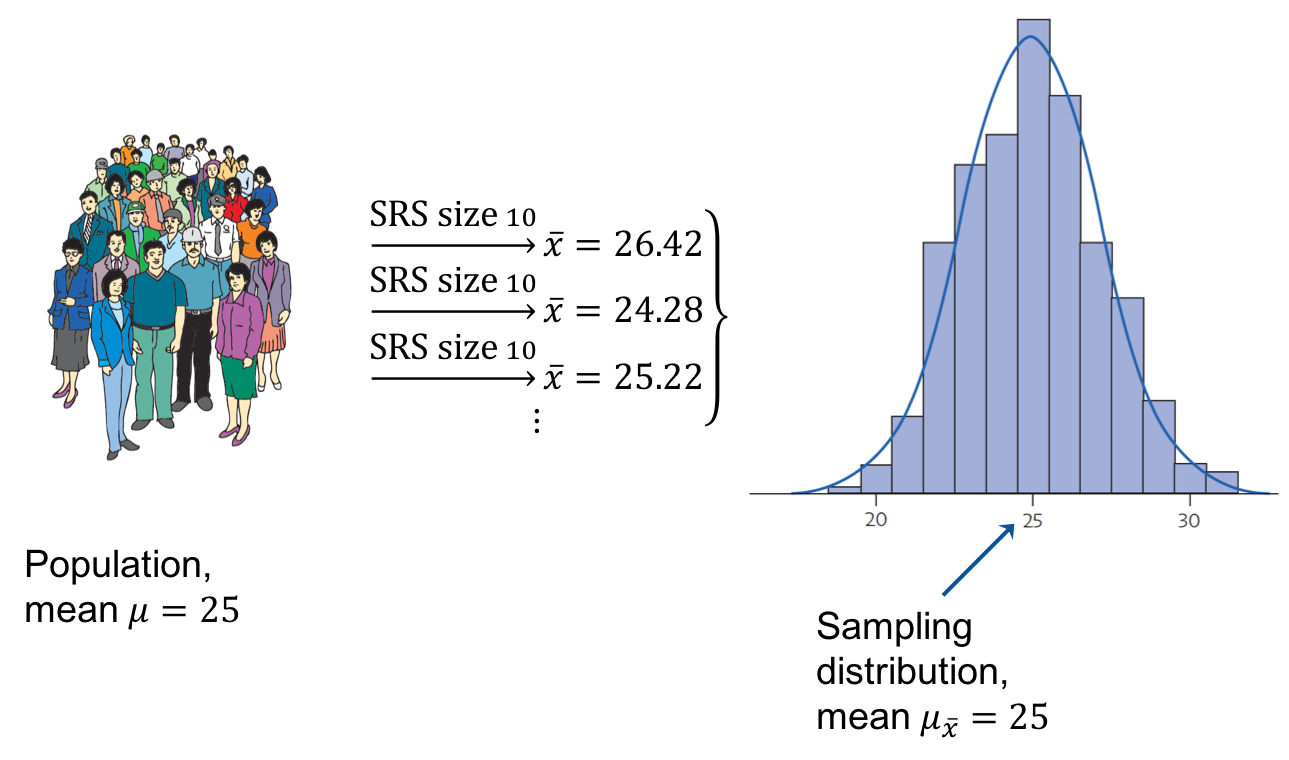
\includegraphics[width=1\textwidth]{samplingdistnofxbar.png}
	\end{center}
\end{frame}

\begin{frame}{Sampling Distributions}
	We will only observe 1 sample in the world though. 
	
	How does the concept of sampling distribution help us?
	\pause
	
	\begin{itemize}
		\item Since we don't know the true population parameter, Our sample statistic will be our best guess at the possible true value.
		
		\item If we know the sampling distribution, then we can consider uncertainty about our sampe statistic.
	\end{itemize}
\end{frame}

\begin{frame}{Law of Large Numbers}
	Under certain conditions, we can use the \alert{Law of Large Numbers (LLN)} to guarantee that $\bar{X}$ approaches $\mu$ as the sample size grows large.
\end{frame}

\begin{frame}{Law of Large Numbers}
	\begin{theorem}[Law of Large Numbers]
		\vspace{2.5mm}
		Let $X_1,X_2,...,X_n$ be an i.i.d. set of observations with $E(X_1) = E(X_2) = ... = E(X_n) = \mu$. Define the sample mean of size $n$ as $\bar{X}_n = \frac{1}{n}\sum_{i = 1}^{n}X_i$. Then
		\[ \bar{X}_n \to \mu \quad \text{as} \quad n \to \infty. \]
	\end{theorem}
	
	Intuitively, as we observe a larger and larger sample, we average over randomness and our sample mean approaches the true population mean. 
\end{frame}


\begin{frame}{Properties of $\bar{X}$}
	\begin{theorem}
		Let $X_1,X_2,...,X_n$ be an i.i.d. sample with $E(X_i) = \mu$ and $Var(X_i) = \sigma^2<\infty$. Then
		\begin{itemize}
			\item $E(\bar{X}) = \mu$,
			\item $Var(\bar{X}) = \frac{\sigma^2}{n}$.
		\end{itemize}
	\end{theorem}
	
	Intuitively, we grab many samples from a population. The variance of our sample averages shrinks as we observe more observations per sample. 
\end{frame}

\begin{frame}{Clicker Question}
	Suppose we sample 100 observations from a distribution with $\mu = 15$ and $\sigma^2 = 25$. What are $E(\bar{X})$ and $Var(\bar{X})$?

	\begin{enumerate}[label=(\alph*)]
		\item $E(\bar{X}) = 15$, $Var(\bar{X}) = 25$.
		\item $E(\bar{X}) = 0.15$, $Var(\bar{X}) = 0.25$.
		\item $E(\bar{X}) = 15$, $Var(\bar{X}) = 5$.
		\item $E(\bar{X}) = 15$, $Var(\bar{X}) = 0.25$.
	\end{enumerate}
\end{frame}


\begin{frame}{When is $\bar{X}$ Normally Distributed?}
	Although we know the mean and variance of $\bar{X}$, we generally don't know its distribution function. 

	\begin{theorem}
		\vspace{2.5mm}
		Let $X_1,X_2,...,X_n$ be an i.i.d. sample with $X_i \sim N(\mu, \sigma^2)$ for $i=1,2,...,n$. 
		
		Then $$
			\bar{X} \sim N(\mu, \frac{\sigma^2}{n}).
		$$
	\end{theorem}
	
	Intuitively, if all the observations come from the same normal distribution then the sample average is also normally distributed and centered at the true mean.
\end{frame}

\begin{frame}{Central Limit Theorem}
	If the number of observation per sample is large (we will discuss this more later), then we know, that the distribution of $X_i$ doesn't matter, we will always have 
	
	$$
		\bar{X} \sim N(\mu, \frac{\sigma^2}{n}).
	$$ 
\end{frame}





\end{document}